\documentclass{article}
\usepackage[utf8]{inputenc}
\usepackage[T1]{fontenc}
\usepackage{graphicx}
\usepackage{hyperref}
\usepackage{geometry}
\geometry{margin=1in}

\title{CABBALLISTS}
\date{Encyclopaedia Britannica (1771)}

\begin{document}
\maketitle

\section*{Historical source}
\textbf{Entry ID:} \texttt{entry-cabballists-2464} \\
\textbf{Volume ID:} 144133902 \\
\textbf{Character Count:} 781

\subsection*{Extracted Text}
CABBALLISTS, the Jewish doctors who profels the fluly of the cabbals.

In the opinion of thefe men, there is not a word, letter, or accent in the law, without fome mystery in it. The Jies are divided into two general feels, the karaice, who refute to receive either tradition or the talmud, or any thing but the pure text of ferripture; and the rabbinills, or talmudits, who, befedes this, receive the traditions of the ancients, and follow the talmud.

The latter are again divided into two other fields; pure rabbinills, explain the ferripure, in its a rural feeling, by grammar, history, and traditions, and cabbullits, who, to difcover hidden mythical fenles, which, they foppefe God to have coached therein, make all of the cabbals, and the mythical methods at bove mentioned.



\section*{Source record}
\begin{itemize}
\item \textbf{Dataset:} \texttt{NationalLibraryOfScotland/encyclopaedia\_britannica\_illustrated}
\item \textbf{Dataset Revision:} \texttt{309f765b1ecc83e0a7f7762e44b4a927a7555443}
\item \textbf{Page ID:} \texttt{britannica:309f765b1ecc83e0a7f7762e44b4a927a7555443:train:2464} \\
  \textbf{Filename:} \texttt{page-2464-24f450326eee.jpg} \\
  \textbf{Row Index:} 2464 \\
  \textbf{SHA256:} \texttt{24f450326eee13b0...}
\end{itemize}

\begin{figure}[h]
\centering
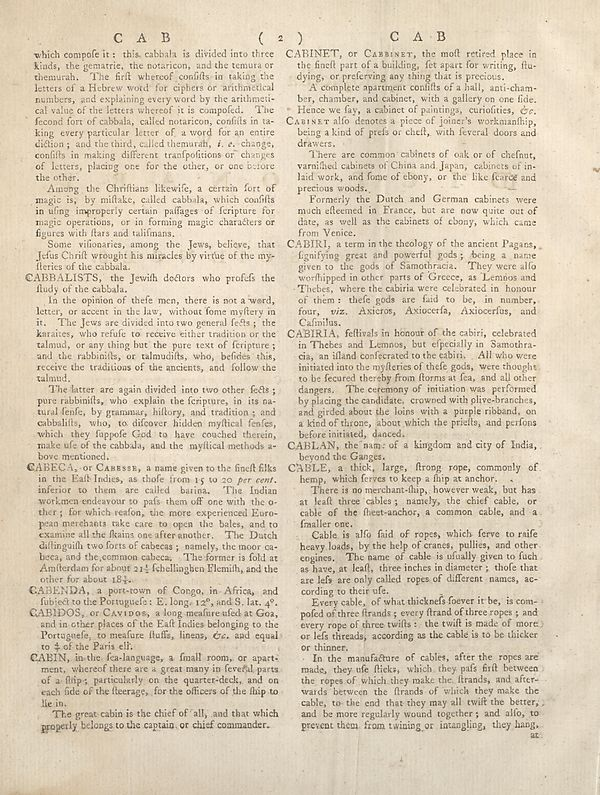
\includegraphics[width=0.85\textwidth]{../scans/page-2464-24f450326eee.jpg}
\caption*{Source scan: \texttt{page-2464-24f450326eee.jpg}}
\end{figure}

\end{document}
